\documentclass{article}
\usepackage{amsmath}
\usepackage{amssymb}
\usepackage{amsthm}
\usepackage{enumerate}
\usepackage{graphicx}
\usepackage{geometry}
\geometry{a4paper, margin=1in}

\title{MIDTERM CHEAT SHEET}
\author{Daniel Palma}
\date{\today}

\begin{document}

\maketitle

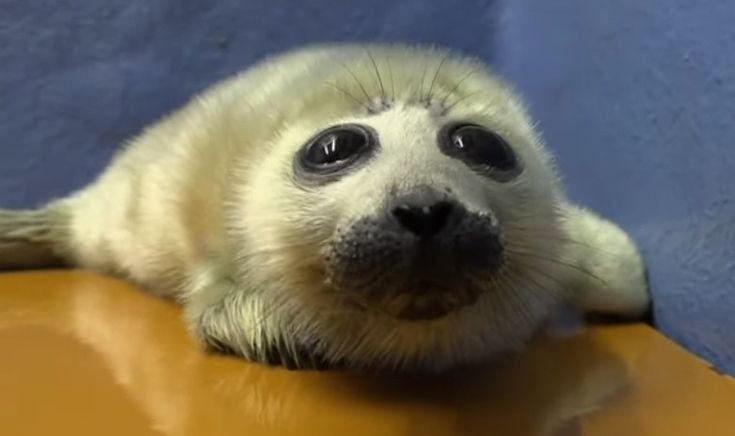
\includegraphics[width=\textwidth]{niko.jpg}

\section{Linear Algebra}

\subsection{Definitions of Matrices and Vectors}
A matrix is a rectangular array of numbers arranged in rows and columns, while a vector is a special case of a matrix with either one row (row vector) or one column (column vector).

\textbf{Notation:} We typically denote matrices with uppercase letters ($A$, $B$, $C$) and vectors with lowercase bold letters ($\mathbf{v}$, $\mathbf{x}$, $\mathbf{y}$).

\textbf{Dimensions:} An $m \times n$ matrix has $m$ rows and $n$ columns.

\textbf{Example expanded:}
\begin{align}
A = \begin{bmatrix} 
1 & 2 \\
3 & 4
\end{bmatrix}, \quad 
\text{Row vector: } \mathbf{a} = \begin{bmatrix} 1 & 2 & 3 \end{bmatrix}, \quad
\text{Column vector: } \mathbf{b} = \begin{bmatrix} 4 \\ 5 \\ 6 \end{bmatrix}
\end{align}

\subsection{Addition, Subtraction, Multiplication}

\subsubsection{Matrix Addition and Subtraction}
Two matrices can be added or subtracted if they have the same dimensions. The operation is performed element-wise.

For matrices $A$ and $B$ of the same dimensions:
\begin{itemize}
    \item Addition: $(A + B)_{ij} = A_{ij} + B_{ij}$
    \item Subtraction: $(A - B)_{ij} = A_{ij} - B_{ij}$
\end{itemize}

\textbf{Example:}
\begin{align}
A = \begin{bmatrix} 
1 & 2 \\
3 & 4
\end{bmatrix}, \quad 
B = \begin{bmatrix} 
5 & 6 \\
7 & 8
\end{bmatrix}, \quad 
A - B = \begin{bmatrix} 
-4 & -4 \\
-4 & -4
\end{bmatrix}
\end{align}

\subsubsection{Scalar Multiplication}
When multiplying a matrix by a scalar (a single number), each element of the matrix is multiplied by that scalar.

For a scalar $c$ and matrix $A$:
\begin{itemize}
    \item Scalar multiplication: $(cA)_{ij} = c \cdot A_{ij}$
\end{itemize}

\textbf{Example:}
\begin{align}
A = \begin{bmatrix} 
1 & 2 \\
3 & 4
\end{bmatrix}, \quad 
3A = \begin{bmatrix} 
3 & 6 \\
9 & 12
\end{bmatrix}
\end{align}

\subsubsection{Matrix Multiplication}
Matrix multiplication is more complex. For two matrices $A$ and $B$ to be multiplied (in the order $A \times B$), the number of columns in $A$ must equal the number of rows in $B$.

If $A$ is an $m \times n$ matrix and $B$ is an $n \times p$ matrix, then $C = A \times B$ is an $m \times p$ matrix.

The $(i,j)$ element of $C$ is:
\begin{align}
C_{ij} = \sum_{k=1}^{n} A_{ik} \cdot B_{kj}
\end{align}

\textbf{Example with steps:}
For $A = \begin{bmatrix} 1 & 2 \\ 3 & 4 \end{bmatrix}$ and $B = \begin{bmatrix} 5 & 6 \\ 7 & 8 \end{bmatrix}$, the multiplication $A \times B$ is:

\begin{align}
C_{11} &= A_{11} \cdot B_{11} + A_{12} \cdot B_{21} = 1 \cdot 5 + 2 \cdot 7 = 5 + 14 = 19\\
C_{12} &= A_{11} \cdot B_{12} + A_{12} \cdot B_{22} = 1 \cdot 6 + 2 \cdot 8 = 6 + 16 = 22\\
C_{21} &= A_{21} \cdot B_{11} + A_{22} \cdot B_{21} = 3 \cdot 5 + 4 \cdot 7 = 15 + 28 = 43\\
C_{22} &= A_{21} \cdot B_{12} + A_{22} \cdot B_{22} = 3 \cdot 6 + 4 \cdot 8 = 18 + 32 = 50
\end{align}

So $A \times B = \begin{bmatrix} 19 & 22 \\ 43 & 50 \end{bmatrix}$

\subsection{Diagonal and Identity Matrices}

A \textbf{diagonal matrix} has non-zero elements only on its main diagonal (from top-left to bottom-right).

A \textbf{identity matrix} (denoted $I$) is a special diagonal matrix with 1s on the main diagonal and 0s elsewhere.

\textbf{Properties:}
\begin{itemize}
    \item For any matrix $A$, $A \cdot I = I \cdot A = A$ (identity property)
    \item Diagonal matrices commute under multiplication: if $D_1$ and $D_2$ are diagonal, then $D_1 \cdot D_2 = D_2 \cdot D_1$
\end{itemize}

\textbf{Example of $3 \times 3$ diagonal and identity matrices:}
\begin{align}
D = \begin{bmatrix} 
4 & 0 & 0 \\
0 & 5 & 0 \\
0 & 0 & 6
\end{bmatrix}, \quad 
I = \begin{bmatrix} 
1 & 0 & 0 \\
0 & 1 & 0 \\
0 & 0 & 1
\end{bmatrix}
\end{align}

\subsection{Determinant and Eigenstructure}

\subsubsection{Determinant}
The determinant is a scalar value associated with a square matrix that has important geometric and algebraic interpretations.

\textbf{Properties of determinants:}
\begin{itemize}
    \item $\det(AB) = \det(A) \cdot \det(B)$
    \item $\det(A^{-1}) = \frac{1}{\det(A)}$
    \item $\det(A^T) = \det(A)$
\end{itemize}

\textbf{Calculation for $3 \times 3$ matrix:}
For $A = \begin{bmatrix} a & b & c \\ d & e & f \\ g & h & i \end{bmatrix}$, the determinant is:
\begin{align}
\det(A) = a(ei - fh) - b(di - fg) + c(dh - eg)
\end{align}

\textbf{Example:}
\begin{align}
A = \begin{bmatrix} 
2 & 0 & 1 \\
3 & 1 & 2 \\
1 & 0 & 3
\end{bmatrix}
\end{align}

\begin{align}
\det(A) &= 2(1 \cdot 3 - 2 \cdot 0) - 0(3 \cdot 3 - 2 \cdot 1) + 1(3 \cdot 0 - 1 \cdot 1)\\
&= 2 \cdot 3 - 0 - 1 = 5
\end{align}

\subsubsection{Eigenvalues and Eigenvectors}
An eigenvector $\mathbf{v}$ of a square matrix $A$ is a non-zero vector that, when multiplied by $A$, yields a scalar multiple of itself: $A\mathbf{v} = \lambda\mathbf{v}$, where $\lambda$ is the corresponding eigenvalue.

\textbf{Finding eigenvalues:}
\begin{enumerate}
    \item Set up the characteristic equation: $\det(A - \lambda I) = 0$
    \item Solve for $\lambda$
\end{enumerate}

\textbf{Finding eigenvectors:}
For each eigenvalue $\lambda$, solve the homogeneous system: $(A - \lambda I)\mathbf{v} = \mathbf{0}$

\textbf{Example:}
For $A = \begin{bmatrix} 3 & 1 \\ 1 & 3 \end{bmatrix}$

\begin{enumerate}
    \item Characteristic equation:
    \begin{align}
    \det\left(\begin{bmatrix} 3-\lambda & 1 \\ 1 & 3-\lambda \end{bmatrix}\right) = (3-\lambda)(3-\lambda) - 1 \cdot 1 = (3-\lambda)^2 - 1 = 0
    \end{align}
    Solving: $(3-\lambda)^2 = 1 \implies 3-\lambda = \pm 1 \implies \lambda = 2$ or $\lambda = 4$

    \item For $\lambda = 2$:
    \begin{align}
    (A - 2I)\mathbf{v} = \begin{bmatrix} 1 & 1 \\ 1 & 1 \end{bmatrix}\mathbf{v} = \mathbf{0}
    \end{align}
    This gives $v_1 = -v_2$, so an eigenvector is $\begin{bmatrix} 1 \\ -1 \end{bmatrix}$

    \item For $\lambda = 4$:
    \begin{align}
    (A - 4I)\mathbf{v} = \begin{bmatrix} -1 & 1 \\ 1 & -1 \end{bmatrix}\mathbf{v} = \mathbf{0}
    \end{align}
    This gives $v_1 = v_2$, so an eigenvector is $\begin{bmatrix} 1 \\ 1 \end{bmatrix}$
\end{enumerate}

\subsection{Inverses and Singularity}

A square matrix $A$ is \textbf{invertible} if there exists a matrix $A^{-1}$ such that $A \cdot A^{-1} = A^{-1} \cdot A = I$.

\textbf{Conditions for invertibility:}
\begin{itemize}
    \item $A$ is invertible if and only if $\det(A) \neq 0$
    \item If $A$ is not invertible, it is called \textbf{singular}
\end{itemize}

\textbf{Calculating the inverse of a $2 \times 2$ matrix:}
For $A = \begin{bmatrix} a & b \\ c & d \end{bmatrix}$:
\begin{align}
A^{-1} = \frac{1}{\det(A)} \begin{bmatrix} d & -b \\ -c & a \end{bmatrix} = \frac{1}{ad-bc} \begin{bmatrix} d & -b \\ -c & a \end{bmatrix}
\end{align}

\textbf{Properties:}
\begin{itemize}
    \item $(AB)^{-1} = B^{-1}A^{-1}$
    \item $(A^{-1})^{-1} = A$
    \item $(A^T)^{-1} = (A^{-1})^T$
\end{itemize}

\textbf{Example with a $3 \times 3$ matrix:}
For $A = \begin{bmatrix} 1 & 0 & 2 \\ 0 & 3 & 1 \\ 1 & 1 & 0 \end{bmatrix}$

You can use Gaussian elimination or the formula involving the adjugate to find:
\begin{align}
A^{-1} = \begin{bmatrix} 
-\frac{2}{5} & \frac{2}{5} & \frac{3}{5} \\
\frac{1}{5} & \frac{1}{5} & -\frac{1}{5} \\
\frac{3}{5} & -\frac{1}{5} & -\frac{1}{5}
\end{bmatrix}
\end{align}
Verifying: $A \cdot A^{-1} = I$

\subsection{Systems of Equations}

A system of linear equations can be written in matrix form as $A\mathbf{x} = \mathbf{b}$.

\textbf{Solving methods:}
\begin{enumerate}
    \item \textbf{Direct solution (if $A$ is invertible):} $\mathbf{x} = A^{-1}\mathbf{b}$
    \item \textbf{Gaussian elimination:} Transform the augmented matrix $[A|\mathbf{b}]$ into row echelon form
    \item \textbf{Cramer's rule:} $x_j = \frac{\det(A_j)}{\det(A)}$, where $A_j$ is $A$ with column $j$ replaced by $\mathbf{b}$
\end{enumerate}

\textbf{Example with solution:}
For the system:
\begin{align}
2x + y - z &= 8\\
-3x + y + 2z &= -2\\
x + y + z &= 3
\end{align}

Matrix form:
\begin{align}
\begin{bmatrix} 
2 & 1 & -1 \\
-3 & 1 & 2 \\
1 & 1 & 1
\end{bmatrix}
\begin{bmatrix} x \\ y \\ z \end{bmatrix} = 
\begin{bmatrix} 8 \\ -2 \\ 3 \end{bmatrix}
\end{align}

Using Gaussian elimination:
\begin{align}
\left[\begin{array}{ccc|c}
2 & 1 & -1 & 8 \\
-3 & 1 & 2 & -2 \\
1 & 1 & 1 & 3
\end{array}\right] \rightarrow
\left[\begin{array}{ccc|c}
1 & 0 & 0 & 2 \\
0 & 1 & 0 & 1 \\
0 & 0 & 1 & 0
\end{array}\right]
\end{align}

So the solution is $x = 2$, $y = 1$, $z = 0$.

\subsection{Singular Value Decomposition (SVD)}

SVD states that any $m \times n$ matrix $A$ can be decomposed as:
\begin{align}
A = U\Sigma V^T
\end{align}

Where:
\begin{itemize}
    \item $U$ is an $m \times m$ orthogonal matrix ($UU^T = I$)
    \item $\Sigma$ is an $m \times n$ diagonal matrix with non-negative entries (singular values)
    \item $V$ is an $n \times n$ orthogonal matrix ($VV^T = I$)
\end{itemize}

\textbf{Applications:}
\begin{itemize}
    \item Least squares approximation
    \item Image compression
    \item Principal Component Analysis
    \item Pseudoinverse calculation: $A^+ = V\Sigma^+U^T$, where $\Sigma^+$ is obtained by taking the reciprocal of non-zero singular values
\end{itemize}

\textbf{Example:}
For $A = \begin{bmatrix} 3 & 2 \\ 2 & 3 \end{bmatrix}$, the SVD is:
\begin{align}
U = \begin{bmatrix} 
\frac{1}{\sqrt{2}} & \frac{1}{\sqrt{2}} \\
\frac{1}{\sqrt{2}} & -\frac{1}{\sqrt{2}}
\end{bmatrix}, \quad
\Sigma = \begin{bmatrix} 
5 & 0 \\
0 & 1
\end{bmatrix}, \quad
V = \begin{bmatrix} 
\frac{1}{\sqrt{2}} & \frac{1}{\sqrt{2}} \\
\frac{1}{\sqrt{2}} & -\frac{1}{\sqrt{2}}
\end{bmatrix}
\end{align}

\subsection{Spectral Decomposition}

For a square matrix $A$ with $n$ linearly independent eigenvectors, the spectral decomposition is:
\begin{align}
A = PDP^{-1}
\end{align}

Where:
\begin{itemize}
    \item $P$ is the matrix of eigenvectors
    \item $D$ is a diagonal matrix of eigenvalues
\end{itemize}

\textbf{Applications:}
\begin{itemize}
    \item Computing matrix powers: $A^k = PD^kP^{-1}$
    \item Solving differential equations
    \item Analyzing dynamical systems
\end{itemize}

\textbf{Example:}
For $A = \begin{bmatrix} 3 & 1 \\ 1 & 3 \end{bmatrix}$ from our eigenvalue example:
\begin{align}
P = \begin{bmatrix} 
1 & 1 \\
-1 & 1
\end{bmatrix}, \quad
D = \begin{bmatrix} 
2 & 0 \\
0 & 4
\end{bmatrix}, \quad
P^{-1} = \begin{bmatrix} 
\frac{1}{2} & -\frac{1}{2} \\
-\frac{1}{2} & \frac{1}{2}
\end{bmatrix}
\end{align}

\subsection{Properties and Derivations of Matrix Traces}

The trace of a square matrix $A$, denoted $\text{tr}(A)$, is the sum of its diagonal elements.

\textbf{Properties:}
\begin{itemize}
    \item $\text{tr}(A + B) = \text{tr}(A) + \text{tr}(B)$
    \item $\text{tr}(cA) = c \cdot \text{tr}(A)$ for scalar $c$
    \item $\text{tr}(AB) = \text{tr}(BA)$, even when $A$ and $B$ have different dimensions (as long as both products are defined)
    \item $\text{tr}(A) =$ sum of eigenvalues of $A$
    \item For orthogonal matrices $Q$, $\text{tr}(Q^TAQ) = \text{tr}(A)$
\end{itemize}

\textbf{Applications:}
\begin{itemize}
    \item In statistics: $\text{tr}(\Sigma\Sigma^T)$ represents the total variance in multivariate analysis
    \item In optimization: many objective functions involve traces
    \item In physics: traces appear in quantum mechanics
\end{itemize}

\textbf{Example with matrix products:}
\begin{align}
A &= \begin{bmatrix} 1 & 2 \\ 3 & 4 \end{bmatrix}, \quad
B = \begin{bmatrix} 5 & 6 \\ 7 & 8 \end{bmatrix}\\
\text{tr}(A) &= 1 + 4 = 5\\
\text{tr}(B) &= 5 + 8 = 13\\
\text{tr}(AB) &= \text{tr}\left(\begin{bmatrix} 19 & 22 \\ 43 & 50 \end{bmatrix}\right) = 19 + 50 = 69
\end{align}

Also:
\begin{align}
BA &= \begin{bmatrix} 5 & 6 \\ 7 & 8 \end{bmatrix} \begin{bmatrix} 1 & 2 \\ 3 & 4 \end{bmatrix} = \begin{bmatrix} 23 & 34 \\ 31 & 46 \end{bmatrix}\\
\text{tr}(BA) &= 23 + 46 = 69 = \text{tr}(AB)
\end{align}

This demonstrates the property that $\text{tr}(AB) = \text{tr}(BA)$.

\section{Machine Learning}

\subsection{Framework for Classical Machine Learning}
\begin{itemize}
    \item \textbf{Definition}: Classical machine learning involves training models on labeled data to make predictions or decisions without being explicitly programmed. These algorithms identify patterns in data through statistical techniques and use these patterns to make predictions on new, unseen data. The learning process often involves optimizing a mathematical function that measures how well the model performs.
    
    \item \textbf{Key Components}:
    \begin{itemize}
        \item Data: Labeled examples used for training and testing
        \item Features: Measurable properties or characteristics extracted from data
        \item Algorithm: The method used to learn patterns from the data
        \item Model: The representation learned from the data
        \item Evaluation metrics: Methods to assess model performance (accuracy, precision, recall, F1 score)
    \end{itemize}
    
    \item \textbf{Learning Paradigms}:
    \begin{itemize}
        \item Batch learning: Model is trained on the entire dataset at once
        \item Online learning: Model is updated incrementally as new data arrives
    \end{itemize}
    
    \item \textbf{Examples}:
    \begin{itemize}
        \item Linear regression for predicting continuous values
        \item Decision trees for classification and regression
        \item Support vector machines for classification using optimal hyperplanes
        \item Random forests for ensemble learning
        \item k-nearest neighbors for instance-based learning
        \item Naive Bayes for probabilistic classification
    \end{itemize}
    
    \item \textbf{The Curse of Dimensionality}:
    \begin{itemize}
        \item Definition: Refers to various phenomena that arise when analyzing data in high-dimensional spaces that do not occur in lower-dimensional settings
        \item Key challenges:
        \begin{itemize}
            \item Exponential growth in volume: As dimensionality increases, the volume of the space increases exponentially, making data increasingly sparse
            \item Distance concentration: In high-dimensional spaces, distances between points become more similar, reducing the effectiveness of distance-based algorithms
            \item Sample size requirements: The amount of data needed to achieve statistical significance grows exponentially with dimensions
            \item Computational complexity: Processing high-dimensional data requires significantly more computational resources
        \end{itemize}
        \item Practical implications:
        \begin{itemize}
            \item Models require exponentially more training data as dimensions increase
            \item Feature selection and dimensionality reduction become essential
            \item Models more prone to overfitting in high-dimensional spaces
            \item Intuition from low-dimensional spaces often fails in high dimensions
        \end{itemize}
    \end{itemize}
\end{itemize}

\subsection{Framework for Deep Learning}
\begin{itemize}
    \item \textbf{Definition}: Deep learning uses neural networks with multiple layers to learn complex patterns in data. It is a subset of machine learning that focuses on learning hierarchical representations directly from raw data, eliminating the need for manual feature engineering. The "deep" refers to the use of multiple layers in the neural network.
    
    \item \textbf{Key Components}:
    \begin{itemize}
        \item Neural network architecture: Organization of neurons and connections
        \item Activation functions: Non-linear transformations applied to neuron outputs (ReLU, sigmoid, tanh)
        \item Loss functions: Measures how well the model performs (cross-entropy, mean squared error)
        \item Optimizers: Algorithms that update model parameters (Adam, SGD, RMSprop)
        \item Regularization techniques: Methods to prevent overfitting (dropout, batch normalization)
    \end{itemize}
    
    \item \textbf{Types of Architectures}:
    \begin{itemize}
        \item Feedforward Neural Networks: Basic architecture where information flows in one direction
        \item Convolutional Neural Networks (CNNs): Specialized for grid-like data such as images
        \item Recurrent Neural Networks (RNNs): For sequential data with LSTM/GRU variants
        \item Transformers: Self-attention based models for sequence processing
        \item Generative Adversarial Networks (GANs): For generating new data samples
        \item Autoencoders: For unsupervised feature learning and dimensionality reduction
    \end{itemize}
    
    \item \textbf{Applications}:
    \begin{itemize}
        \item Computer vision (object detection, image recognition)
        \item Natural language processing (translation, sentiment analysis)
        \item Speech recognition and synthesis
        \item Game playing (AlphaGo, chess)
        \item Drug discovery and molecular design
    \end{itemize}
    
    \item \textbf{Overfitting in Deep Learning}:
    \begin{itemize}
        \item Definition: Overfitting occurs when a model learns the training data too well, capturing noise and specific details rather than general patterns, resulting in poor generalization to new data.
        
        \item Characteristics of overfitting:
        \begin{itemize}
            \item High accuracy on training data but poor performance on test data
            \item Complex model with many parameters relative to the amount of training data
            \item Model captures random fluctuations in the training data
        \end{itemize}
        
        \item Solutions to overfitting:
        \begin{itemize}
            \item Regularization techniques: L1/L2 regularization to penalize large weights
            \item Dropout: Randomly disabling neurons during training
            \item Early stopping: Halting training when validation performance starts to degrade
            \item Data augmentation: Creating variations of training examples
            \item Batch normalization: Normalizing inputs to each layer
            \item Transfer learning: Using pre-trained models as starting points
        \end{itemize}
    \end{itemize}
\end{itemize}

\subsection{Supervised Learning Formulations}
\begin{itemize}
    \item \textbf{Definition}: Supervised learning involves learning a mapping function from input variables (X) to output variables (Y) using labeled training data. The goal is to approximate this mapping function so well that when given new input data, the model can predict the output variables.
    
    \item \textbf{Mathematical Formulation}:
    \begin{itemize}
        \item Input space: X (features)
        \item Output space: Y (labels/targets)
        \item Training data: $D = \{(x_1, y_1), (x_2, y_2), ..., (x_n, y_n)\}$
        \item Hypothesis space: H (set of possible mapping functions)
        \item Goal: Find h $\in$ H such that h: X $\rightarrow$ Y minimizes the expected loss
    \end{itemize}
    
    \item \textbf{Loss Functions}:
    \begin{itemize}
        \item Regression: Mean Squared Error (MSE), Mean Absolute Error (MAE)
        \item Classification: Cross-Entropy Loss, Hinge Loss, Log Loss
    \end{itemize}
    
    \item \textbf{Types of Supervised Learning}:
    \begin{itemize}
        \item Classification: Predicting discrete class labels
        \begin{itemize}
            \item Binary classification (spam detection, disease diagnosis)
            \item Multi-class classification (digit recognition, species identification)
            \item Multi-label classification (tagging images with multiple concepts)
        \end{itemize}
        
        \item Regression: Predicting continuous values
        \begin{itemize}
            \item Simple linear regression (one feature)
            \item Multiple linear regression (multiple features)
            \item Polynomial regression (non-linear relationships)
            \item Support vector regression (using kernel methods)
        \end{itemize}
    \end{itemize}
    
    \item \textbf{Examples}:
    \begin{itemize}
        \item Predicting house prices based on features like size, location, age
        \item Email spam detection
        \item Medical diagnosis
        \item Credit risk assessment
        \item Image recognition
    \end{itemize}
    
    \item \textbf{Stochastic Gradient Descent (SGD)}:
    \begin{itemize}
        \item Definition: SGD is an optimization algorithm used to find the parameters that minimize the loss function in supervised learning.
        
        \item Mathematical Definition:
        \begin{itemize}
            \item For a loss function L($\theta$) with parameters $\theta$:
            \begin{enumerate}
                \item Initialize parameters $\theta_0$
                \item For each iteration t = 1, 2, ..., T:
                \begin{itemize}
                    \item Randomly select a mini-batch of m samples
                    \item Compute gradient: $g_t = \nabla_\theta L(\theta_{t-1}; x_i, y_i)$ for samples in mini-batch
                    \item Update parameters: $\theta_t = \theta_{t-1} - \eta_t \cdot g_t$
                    \item where $\eta_t$ is the learning rate at iteration t
                \end{itemize}
            \end{enumerate}
        \end{itemize}
        
        \item Formula:
        \begin{itemize}
            \item $\theta_t = \theta_{t-1} - \eta_t \cdot \nabla_\theta L(\theta_{t-1}; x_i, y_i)$
        \end{itemize}
        
        \item Key characteristics:
        \begin{itemize}
            \item Uses a subset of training examples (mini-batch) for each update
            \item More computationally efficient than batch gradient descent
            \item Introduces noise in the gradient, which can help escape local minima
            \item Requires tuning of hyperparameters like learning rate and batch size
            \item Variants include momentum SGD, Adam, RMSprop, and AdaGrad
        \end{itemize}
        
        \item Advantages:
        \begin{itemize}
            \item Faster convergence for large datasets
            \item Lower memory requirements
            \item May provide better generalization due to noise in updates
            \item More likely to escape shallow local minima
        \end{itemize}
    \end{itemize}
\end{itemize}

\subsection{Asymptotic Analysis}
\begin{itemize}
    \item \textbf{Definition}: Asymptotic analysis studies the behavior of algorithms and functions as the input size approaches infinity. It provides a mathematical framework for describing the efficiency of algorithms independent of hardware or implementation details.
    
    \item \textbf{Key Concepts}:
    \begin{itemize}
        \item Big-O notation (O): Upper bound on growth rate
        \begin{itemize}
            \item f(n) = O(g(n)) if there exist constants c > 0 and $n_0$ such that 0 $\leq$ f(n) $\leq$ c$\cdot$g(n) for all n $\geq$ $n_0$
        \end{itemize}
        
        \item Big-Omega notation ($\Omega$): Lower bound on growth rate
        \begin{itemize}
            \item f(n) = $\Omega$(g(n)) if there exist constants c > 0 and $n_0$ such that 0 $\leq$ c$\cdot$g(n) $\leq$ f(n) for all n $\geq$ $n_0$
        \end{itemize}
        
        \item Big-Theta notation ($\Theta$): Tight bound on growth rate
        \begin{itemize}
            \item f(n) = $\Theta$(g(n)) if f(n) = O(g(n)) and f(n) = $\Omega$(g(n))
        \end{itemize}
    \end{itemize}
    
    \item \textbf{Common Complexities}:
    \begin{itemize}
        \item O(1): Constant time (hash table lookups)
        \item O(log n): Logarithmic (binary search)
        \item O(n): Linear (linear search)
        \item O(n log n): Log-linear (efficient sorting algorithms)
        \item O($n^2$): Quadratic (simple sorting algorithms)
        \item O($2^n$): Exponential (brute force algorithms)
    \end{itemize}
    
    \item \textbf{Applications in Machine Learning}:
    \begin{itemize}
        \item Analyzing time complexity of training algorithms
        \item Evaluating scalability with increasing data dimensions
        \item Determining computational feasibility for large datasets
        \item Comparing efficiency of different learning algorithms
    \end{itemize}
    
    \item \textbf{Examples}:
    \begin{itemize}
        \item k-nearest neighbors has O(nd) query time complexity, where n is the number of samples and d is the number of dimensions
        \item Decision tree induction has O(d n log n) complexity for n samples with d dimensions
        \item Neural network training with SGD has O(n d w) complexity per epoch, where n is the number of samples, d is the dimension, and w is the number of weights
    \end{itemize}
\end{itemize}

\subsection{Non-asymptotic Analysis}
\begin{itemize}
    \item \textbf{Definition}: Non-asymptotic analysis focuses on the performance of algorithms for finite input sizes, providing explicit bounds that hold for any sample size rather than just asymptotic behavior.
    
    \item \textbf{Key Concepts}:
    \begin{itemize}
        \item Concentration inequalities: Bounds on how a random variable deviates from its expected value
        \item High-probability bounds: Guarantees that hold with high probability but not necessarily always
        \item Uniform convergence: Convergence that applies simultaneously to all functions in a class
        \item Generalization error bounds: Limits on the difference between training and test performance
    \end{itemize}
    
    \item \textbf{Important Tools}:
    \begin{itemize}
        \item Hoeffding's inequality: Bounds the probability that the sum of bounded random variables deviates from its expected value
        \item Markov's inequality: Provides bounds for non-negative random variables
        \item Chebyshev's inequality: Relates variance to probability of deviation from the mean
        \item McDiarmid's inequality: Bounds for functions of independent random variables
        \item VC dimension: Measure of complexity for hypothesis classes
    \end{itemize}
    
    \item \textbf{Applications in Machine Learning}:
    \begin{itemize}
        \item Deriving sample complexity: Number of samples needed to achieve a specific error rate
        \item Bounding generalization error: Gap between training and test performance
        \item Model selection: Choosing between different model complexities
        \item Early stopping criteria: Deciding when to halt the training process
        \item Regularization parameter selection: Determining optimal strength of regularization
    \end{itemize}
    
    \item \textbf{Examples}:
    \begin{itemize}
        \item For empirical risk minimization, the generalization error is bounded by O($\sqrt{\frac{\log(1/\delta)}{n}}$) with probability 1-$\delta$
        \item VC dimension-based bounds show that the sample complexity scales linearly with the VC dimension
        \item Rademacher complexity provides data-dependent bounds on the generalization error
        \item PAC learning theory provides bounds on the sample complexity needed to learn a concept with high probability
    \end{itemize}
\end{itemize}

\section{Python Data Types}

\subsection{Overview of Python Data Types}
\begin{itemize}
    \item Python provides a variety of built-in data types, categorized into mutable and immutable types.
    \item Mutable types can be modified after creation, while immutable types cannot.
\end{itemize}

\subsection{Immutable Data Types}
\begin{itemize}
    \item \textbf{Integers (int)}
    \begin{itemize}
        \item Whole numbers, positive or negative.
        \item Arbitrary-precision arithmetic.
        \item Example: \texttt{x = 42}
    \end{itemize}
    \item \textbf{Floating-Point Numbers (float)}
    \begin{itemize}
        \item Decimal numbers with fractional parts.
        \item Example: \texttt{y = 3.14}
    \end{itemize}
    \item \textbf{Complex Numbers (complex)}
    \begin{itemize}
        \item Numbers with real and imaginary parts.
        \item Example: \texttt{z = 3 + 4j}
    \end{itemize}
    \item \textbf{Strings (str)}
    \begin{itemize}
        \item Sequence of Unicode characters.
        \item Immutable.
        \item Example: \texttt{text = "Hello"}
    \end{itemize}
    \item \textbf{Tuples (tuple)}
    \begin{itemize}
        \item Ordered collection of elements.
        \item Immutable.
        \item Example: \texttt{t = (1, 2, 3)}
    \end{itemize}
    \item \textbf{Booleans (bool)}
    \begin{itemize}
        \item Represents True or False values.
        \item Example: \texttt{flag = True}
    \end{itemize}
\end{itemize}

\subsection{Mutable Data Types}
\begin{itemize}
    \item \textbf{Lists (list)}
    \begin{itemize}
        \item Ordered collection of elements.
        \item Mutable (can be modified after creation).
        \item Example: \texttt{lst = [1, 2, 3]}
    \end{itemize}
    \item \textbf{Dictionaries (dict)}
    \begin{itemize}
        \item Key-value pairs.
        \item Mutable.
        \item Example: \texttt{d = \{'a': 1, 'b': 2\}}
    \end{itemize}
    \item \textbf{Sets (set)}
    \begin{itemize}
        \item Unordered collection of unique elements.
        \item Mutable.
        \item Example: \texttt{s = \{1, 2, 3\}}
    \end{itemize}
\end{itemize}

\subsection{Type Conversion}
\begin{itemize}
    \item Python supports explicit and implicit type conversion.
    \item Example:
    \begin{itemize}
        \item Explicit: \texttt{float(5) \# Converts integer 5 to float 5.0}
        \item Implicit: \texttt{x = 5 + 3.2 \# Integer 5 is converted to float}
    \end{itemize}
\end{itemize}

\subsection{Special Data Types}
\begin{itemize}
    \item \textbf{Bytes (bytes)}
    \begin{itemize}
        \item Immutable sequence of bytes.
        \item Example: \texttt{b = b'hello'}
    \end{itemize}
    \item \textbf{Byte Arrays (bytearray)}
    \begin{itemize}
        \item Mutable sequence of bytes.
        \item Example: \texttt{ba = bytearray(5)}
    \end{itemize}
    \item \textbf{NoneType (None)}
    \begin{itemize}
        \item Represents absence of value.
        \item Example: \texttt{x = None}
    \end{itemize}
\end{itemize}


\end{document}